
% This LaTeX was auto-generated from MATLAB code.
% To make changes, update the MATLAB code and republish this document.

\documentclass{article}
\usepackage{graphicx}
\usepackage{color}

\sloppy
\definecolor{lightgray}{gray}{0.5}
\setlength{\parindent}{0pt}

\begin{document}

    
    
\section*{Variational Gradient Matching for Dynamical Systems: Lorenz 96}


\subsection*{Contents}

\begin{itemize}
\setlength{\itemsep}{-1ex}
   \item .
   \item \textbf{Authors}:
   \item Contents:
   \item User Input: Simulation Settings
   \item User Input: Estimation
   \item Preprocessing
   \item Mass Action Dynamical Systems
   \item Simulate Trajectories
   \item Prior on States and State Derivatives
   \item Matching Gradients
   \item Rewrite ODEs as Linear Combination in Parameters
   \item Posterior over ODE Parameters
   \item Rewrite ODEs as Linear Combination in Individual States
   \item Posterior over Individual States
   \item Mean-field Variational Inference
   \item Fitting observations of state trajectories
   \item Coordinate Ascent Variational Gradient Matching
   \item Time Taken
   \item References
\end{itemize}


\subsection*{.}



\subsection*{\textbf{Authors}:}

\begin{par}
\textbf{Nico Stephan Gorbach} and \textbf{Stefan Bauer}, email: \begin{verbatim}nico.gorbach@gmail.com\end{verbatim}
\end{par} \vspace{1em}


\subsection*{Contents:}

\begin{par}
Instructional code for the NIPS (2018) paper \begin{verbatim}Scalable Variational Inference for Dynamical Systems\end{verbatim} by Nico S. Gorbach, Stefan Bauer and Joachim M. Buhmann. Please cite our paper if you use our program for a further publication. Part of the derivation below is described in Wenk et al. (2018).
\end{par} \vspace{1em}
\begin{par}
Example dynamical system used in this code: \textbf{Lorenz 96} system with a \textbf{100 ODEs, with half *of the states *unobserved}. The ODE parameter is also unobserved.
\end{par} \vspace{1em}


\subsection*{User Input: Simulation Settings}

\begin{par}

\end{par} \vspace{1em}
\begin{itemize}
\setlength{\itemsep}{-1ex}
   \item \textbf{true ODE parameter}
\end{itemize}
\begin{itemize}
\setlength{\itemsep}{-1ex}
   \item *               Input a real number:
\end{itemize}
\begin{verbatim}
        simulation.ode_param = 8;
\end{verbatim}
\begin{par}

\end{par} \vspace{1em}
\begin{itemize}
\setlength{\itemsep}{-1ex}
   \item \textbf{number of ODEs}
\end{itemize}
\begin{itemize}
\setlength{\itemsep}{-1ex}
   \item *Input a positive integer:
\end{itemize}
\begin{verbatim}
        simulation.numb_odes = 100;
\end{verbatim}
\begin{par}

\end{par} \vspace{1em}
\begin{itemize}
\setlength{\itemsep}{-1ex}
   \item \textbf{ratio of number of observed states over number of unobserved states}
\end{itemize}

\begin{verbatim}               Input a real number in the interval $(0,1]$:\end{verbatim}
    \begin{verbatim}
        simulation.observed_states = 0.5;    % only 50% of the states are observed
\end{verbatim}
\begin{par}

\end{par} \vspace{1em}
\begin{itemize}
\setlength{\itemsep}{-1ex}
   \item \textbf{observation noise}
\end{itemize}
\begin{itemize}
\setlength{\itemsep}{-1ex}
   \item *Input a function handle:
\end{itemize}
\begin{verbatim}
        simulation.state_obs_variance = @(mean)(bsxfun(@times,0.1,ones(size(mean))));
\end{verbatim}
\begin{par}

\end{par} \vspace{1em}
\begin{itemize}
\setlength{\itemsep}{-1ex}
   \item \textbf{time interval between observations}
\end{itemize}

\begin{verbatim}               Input a positive real number:\end{verbatim}
    \begin{verbatim}
        simulation.interval_between_observations = 0.1;
\end{verbatim}


\subsection*{User Input: Estimation}

\begin{itemize}
\setlength{\itemsep}{-1ex}
   \item *Kernel parameters *\$\ensuremath{\backslash}mathbf\ensuremath{\backslash}phi\$
\end{itemize}

\begin{verbatim}                   Input a row vector of positive real numbers of size
1 x 2:\end{verbatim}
    \begin{verbatim}
        kernel.param = [10,0.2];
\end{verbatim}
\begin{par}

\end{par} \vspace{1em}
\begin{itemize}
\setlength{\itemsep}{-1ex}
   \item \textbf{Error variance on state derivatives (i.e.} $\gamma$*)*
\end{itemize}

\begin{verbatim}                   Input a row vector of positive real numbers of size
1 x number of ODEs:\end{verbatim}
    \begin{verbatim}
        state.derivative_variance = 6*ones(1,simulation.numb_odes);
\end{verbatim}
\begin{par}

\end{par} \vspace{1em}
\begin{itemize}
\setlength{\itemsep}{-1ex}
   \item \textbf{Estimation times}
\end{itemize}

\begin{verbatim}                   Input a row vector of positive real numbers in ascending
order:\end{verbatim}
    \begin{verbatim}
        time.est = 0:0.1:4;
\end{verbatim}
\begin{par}
Preliminary operations
\end{par} \vspace{1em}
\begin{verbatim}
close all; clc; addpath('VGM_functions');
\end{verbatim}


\subsection*{Preprocessing}

\begin{verbatim}
[symbols,simulation,ode,odes_path,coupling_idx,opt_settings,plot_settings] = proprocessing_Lorenz96(simulation);
\end{verbatim}

        \color{lightgray} \begin{verbatim} 
ODEs:
 
/   d x_1                                      \
|   ----- == alpha - x_1 + x_100 (x_2 - x_99)  |
|     dt                                       |
|                                              |
|   d x_2                                      |
|   ----- == alpha - x_2 + x_1 (x_3 - x_100)   |
|     dt                                       |
|                                              |
|    d x_3                                     |
|    ----- == alpha - x_3 - x_2 (x_1 - x_4)    |
|      dt                                      |
|                                              |
|    d x_4                                     |
|    ----- == alpha - x_4 - x_3 (x_2 - x_5)    |
|      dt                                      |
|                                              |
|    d x_5                                     |
|    ----- == alpha - x_5 - x_4 (x_3 - x_6)    |
|      dt                                      |
|                                              |
|    d x_6                                     |
|    ----- == alpha - x_6 - x_5 (x_4 - x_7)    |
|      dt                                      |
|                                              |
|    d x_7                                     |
|    ----- == alpha - x_7 - x_6 (x_5 - x_8)    |
|      dt                                      |
|                                              |
|    d x_8                                     |
|    ----- == alpha - x_8 - x_7 (x_6 - x_9)    |
|      dt                                      |
|                                              |
|    d x_9                                     |
|    ----- == alpha - x_9 - x_8 (x_7 - x_10)   |
|      dt                                      |
|                                              |
|   d x_10                                     |
|   ------ == alpha - x_10 - x_9 (x_8 - x_11)  |
|     dt                                       |
|                                              |
|  d x_11                                      |
|  ------ == alpha - x_11 - x_10 (x_9 - x_12)  |
|    dt                                        |
|                                              |
|  d x_12                                      |
|  ------ == alpha - x_12 - x_11 (x_10 - x_13) |
|    dt                                        |
|                                              |
|  d x_13                                      |
|  ------ == alpha - x_13 - x_12 (x_11 - x_14) |
|    dt                                        |
|                                              |
|  d x_14                                      |
|  ------ == alpha - x_14 - x_13 (x_12 - x_15) |
|    dt                                        |
|                                              |
|  d x_15                                      |
|  ------ == alpha - x_15 - x_14 (x_13 - x_16) |
|    dt                                        |
|                                              |
|  d x_16                                      |
|  ------ == alpha - x_16 - x_15 (x_14 - x_17) |
|    dt                                        |
|                                              |
|  d x_17                                      |
|  ------ == alpha - x_17 - x_16 (x_15 - x_18) |
|    dt                                        |
|                                              |
|  d x_18                                      |
|  ------ == alpha - x_18 - x_17 (x_16 - x_19) |
|    dt                                        |
|                                              |
|  d x_19                                      |
|  ------ == alpha - x_19 - x_18 (x_17 - x_20) |
|    dt                                        |
|                                              |
|  d x_20                                      |
|  ------ == alpha - x_20 - x_19 (x_18 - x_21) |
|    dt                                        |
|                                              |
|  d x_21                                      |
|  ------ == alpha - x_21 - x_20 (x_19 - x_22) |
|    dt                                        |
|                                              |
|  d x_22                                      |
|  ------ == alpha - x_22 - x_21 (x_20 - x_23) |
|    dt                                        |
|                                              |
|  d x_23                                      |
|  ------ == alpha - x_23 - x_22 (x_21 - x_24) |
|    dt                                        |
|                                              |
|  d x_24                                      |
|  ------ == alpha - x_24 - x_23 (x_22 - x_25) |
|    dt                                        |
|                                              |
|  d x_25                                      |
|  ------ == alpha - x_25 - x_24 (x_23 - x_26) |
|    dt                                        |
|                                              |
|  d x_26                                      |
|  ------ == alpha - x_26 - x_25 (x_24 - x_27) |
|    dt                                        |
|                                              |
|  d x_27                                      |
|  ------ == alpha - x_27 - x_26 (x_25 - x_28) |
|    dt                                        |
|                                              |
|  d x_28                                      |
|  ------ == alpha - x_28 - x_27 (x_26 - x_29) |
|    dt                                        |
|                                              |
|  d x_29                                      |
|  ------ == alpha - x_29 - x_28 (x_27 - x_30) |
|    dt                                        |
|                                              |
|  d x_30                                      |
|  ------ == alpha - x_30 - x_29 (x_28 - x_31) |
|    dt                                        |
|                                              |
|  d x_31                                      |
|  ------ == alpha - x_31 - x_30 (x_29 - x_32) |
|    dt                                        |
|                                              |
|  d x_32                                      |
|  ------ == alpha - x_32 - x_31 (x_30 - x_33) |
|    dt                                        |
|                                              |
|  d x_33                                      |
|  ------ == alpha - x_33 - x_32 (x_31 - x_34) |
|    dt                                        |
|                                              |
|  d x_34                                      |
|  ------ == alpha - x_34 - x_33 (x_32 - x_35) |
|    dt                                        |
|                                              |
|  d x_35                                      |
|  ------ == alpha - x_35 - x_34 (x_33 - x_36) |
|    dt                                        |
|                                              |
|  d x_36                                      |
|  ------ == alpha - x_36 - x_35 (x_34 - x_37) |
|    dt                                        |
|                                              |
|  d x_37                                      |
|  ------ == alpha - x_37 - x_36 (x_35 - x_38) |
|    dt                                        |
|                                              |
|  d x_38                                      |
|  ------ == alpha - x_38 - x_37 (x_36 - x_39) |
|    dt                                        |
|                                              |
|  d x_39                                      |
|  ------ == alpha - x_39 - x_38 (x_37 - x_40) |
|    dt                                        |
|                                              |
|  d x_40                                      |
|  ------ == alpha - x_40 - x_39 (x_38 - x_41) |
|    dt                                        |
|                                              |
|  d x_41                                      |
|  ------ == alpha - x_41 - x_40 (x_39 - x_42) |
|    dt                                        |
|                                              |
|  d x_42                                      |
|  ------ == alpha - x_42 - x_41 (x_40 - x_43) |
|    dt                                        |
|                                              |
|  d x_43                                      |
|  ------ == alpha - x_43 - x_42 (x_41 - x_44) |
|    dt                                        |
|                                              |
|  d x_44                                      |
|  ------ == alpha - x_44 - x_43 (x_42 - x_45) |
|    dt                                        |
|                                              |
|  d x_45                                      |
|  ------ == alpha - x_45 - x_44 (x_43 - x_46) |
|    dt                                        |
|                                              |
|  d x_46                                      |
|  ------ == alpha - x_46 - x_45 (x_44 - x_47) |
|    dt                                        |
|                                              |
|  d x_47                                      |
|  ------ == alpha - x_47 - x_46 (x_45 - x_48) |
|    dt                                        |
|                                              |
|  d x_48                                      |
|  ------ == alpha - x_48 - x_47 (x_46 - x_49) |
|    dt                                        |
|                                              |
|  d x_49                                      |
|  ------ == alpha - x_49 - x_48 (x_47 - x_50) |
|    dt                                        |
|                                              |
|  d x_50                                      |
|  ------ == alpha - x_50 - x_49 (x_48 - x_51) |
|    dt                                        |
|                                              |
|  d x_51                                      |
|  ------ == alpha - x_51 - x_50 (x_49 - x_52) |
|    dt                                        |
|                                              |
|  d x_52                                      |
|  ------ == alpha - x_52 - x_51 (x_50 - x_53) |
|    dt                                        |
|                                              |
|  d x_53                                      |
|  ------ == alpha - x_53 - x_52 (x_51 - x_54) |
|    dt                                        |
|                                              |
|  d x_54                                      |
|  ------ == alpha - x_54 - x_53 (x_52 - x_55) |
|    dt                                        |
|                                              |
|  d x_55                                      |
|  ------ == alpha - x_55 - x_54 (x_53 - x_56) |
|    dt                                        |
|                                              |
|  d x_56                                      |
|  ------ == alpha - x_56 - x_55 (x_54 - x_57) |
|    dt                                        |
|                                              |
|  d x_57                                      |
|  ------ == alpha - x_57 - x_56 (x_55 - x_58) |
|    dt                                        |
|                                              |
|  d x_58                                      |
|  ------ == alpha - x_58 - x_57 (x_56 - x_59) |
|    dt                                        |
|                                              |
|  d x_59                                      |
|  ------ == alpha - x_59 - x_58 (x_57 - x_60) |
|    dt                                        |
|                                              |
|  d x_60                                      |
|  ------ == alpha - x_60 - x_59 (x_58 - x_61) |
|    dt                                        |
|                                              |
|  d x_61                                      |
|  ------ == alpha - x_61 - x_60 (x_59 - x_62) |
|    dt                                        |
|                                              |
|  d x_62                                      |
|  ------ == alpha - x_62 - x_61 (x_60 - x_63) |
|    dt                                        |
|                                              |
|  d x_63                                      |
|  ------ == alpha - x_63 - x_62 (x_61 - x_64) |
|    dt                                        |
|                                              |
|  d x_64                                      |
|  ------ == alpha - x_64 - x_63 (x_62 - x_65) |
|    dt                                        |
|                                              |
|  d x_65                                      |
|  ------ == alpha - x_65 - x_64 (x_63 - x_66) |
|    dt                                        |
|                                              |
|  d x_66                                      |
|  ------ == alpha - x_66 - x_65 (x_64 - x_67) |
|    dt                                        |
|                                              |
|  d x_67                                      |
|  ------ == alpha - x_67 - x_66 (x_65 - x_68) |
|    dt                                        |
|                                              |
|  d x_68                                      |
|  ------ == alpha - x_68 - x_67 (x_66 - x_69) |
|    dt                                        |
|                                              |
|  d x_69                                      |
|  ------ == alpha - x_69 - x_68 (x_67 - x_70) |
|    dt                                        |
|                                              |
|  d x_70                                      |
|  ------ == alpha - x_70 - x_69 (x_68 - x_71) |
|    dt                                        |
|                                              |
|  d x_71                                      |
|  ------ == alpha - x_71 - x_70 (x_69 - x_72) |
|    dt                                        |
|                                              |
|  d x_72                                      |
|  ------ == alpha - x_72 - x_71 (x_70 - x_73) |
|    dt                                        |
|                                              |
|  d x_73                                      |
|  ------ == alpha - x_73 - x_72 (x_71 - x_74) |
|    dt                                        |
|                                              |
|  d x_74                                      |
|  ------ == alpha - x_74 - x_73 (x_72 - x_75) |
|    dt                                        |
|                                              |
|  d x_75                                      |
|  ------ == alpha - x_75 - x_74 (x_73 - x_76) |
|    dt                                        |
|                                              |
|  d x_76                                      |
|  ------ == alpha - x_76 - x_75 (x_74 - x_77) |
|    dt                                        |
|                                              |
|  d x_77                                      |
|  ------ == alpha - x_77 - x_76 (x_75 - x_78) |
|    dt                                        |
|                                              |
|  d x_78                                      |
|  ------ == alpha - x_78 - x_77 (x_76 - x_79) |
|    dt                                        |
|                                              |
|  d x_79                                      |
|  ------ == alpha - x_79 - x_78 (x_77 - x_80) |
|    dt                                        |
|                                              |
|  d x_80                                      |
|  ------ == alpha - x_80 - x_79 (x_78 - x_81) |
|    dt                                        |
|                                              |
|  d x_81                                      |
|  ------ == alpha - x_81 - x_80 (x_79 - x_82) |
|    dt                                        |
|                                              |
|  d x_82                                      |
|  ------ == alpha - x_82 - x_81 (x_80 - x_83) |
|    dt                                        |
|                                              |
|  d x_83                                      |
|  ------ == alpha - x_83 - x_82 (x_81 - x_84) |
|    dt                                        |
|                                              |
|  d x_84                                      |
|  ------ == alpha - x_84 - x_83 (x_82 - x_85) |
|    dt                                        |
|                                              |
|  d x_85                                      |
|  ------ == alpha - x_85 - x_84 (x_83 - x_86) |
|    dt                                        |
|                                              |
|  d x_86                                      |
|  ------ == alpha - x_86 - x_85 (x_84 - x_87) |
|    dt                                        |
|                                              |
|  d x_87                                      |
|  ------ == alpha - x_87 - x_86 (x_85 - x_88) |
|    dt                                        |
|                                              |
|  d x_88                                      |
|  ------ == alpha - x_88 - x_87 (x_86 - x_89) |
|    dt                                        |
|                                              |
|  d x_89                                      |
|  ------ == alpha - x_89 - x_88 (x_87 - x_90) |
|    dt                                        |
|                                              |
|  d x_90                                      |
|  ------ == alpha - x_90 - x_89 (x_88 - x_91) |
|    dt                                        |
|                                              |
|  d x_91                                      |
|  ------ == alpha - x_91 - x_90 (x_89 - x_92) |
|    dt                                        |
|                                              |
|  d x_92                                      |
|  ------ == alpha - x_92 - x_91 (x_90 - x_93) |
|    dt                                        |
|                                              |
|  d x_93                                      |
|  ------ == alpha - x_93 - x_92 (x_91 - x_94) |
|    dt                                        |
|                                              |
|  d x_94                                      |
|  ------ == alpha - x_94 - x_93 (x_92 - x_95) |
|    dt                                        |
|                                              |
|  d x_95                                      |
|  ------ == alpha - x_95 - x_94 (x_93 - x_96) |
|    dt                                        |
|                                              |
|  d x_96                                      |
|  ------ == alpha - x_96 - x_95 (x_94 - x_97) |
|    dt                                        |
|                                              |
|  d x_97                                      |
|  ------ == alpha - x_97 - x_96 (x_95 - x_98) |
|    dt                                        |
|                                              |
|  d x_98                                      |
|  ------ == alpha - x_98 - x_97 (x_96 - x_99) |
|    dt                                        |
|                                              |
| d x_99                                       |
| ------ == alpha - x_99 - x_98 (x_97 - x_100) |
|   dt                                         |
|                                              |
| d x_100                                      |
| ------- == alpha - x_100 + x_99 (x_1 - x_98) |
\    dt                                        /

\end{verbatim} \color{black}
    

\subsection*{Mass Action Dynamical Systems}

\begin{par}
A deterministic dynamical system is represented by a set of $K$ ordinary differential equations (ODEs) with model parameters $\mathbf\theta \in \mathcal{R}^d$ that describe the evolution of $K$ states $\mathbf{x}(t) = [x_1(t),\ldots, x_K(t)]^T$ such that:
\end{par} \vspace{1em}
\begin{par}
$\dot{\mathbf{x}}(t) = \frac{d \mathbf{x}(t)}{d t} = \mathbf{f}(\mathbf{x}(t),\mathbf\theta) \qquad (1)$,
\end{par} \vspace{1em}
\begin{par}
A sequence of observations, $\mathbf{y}(t)$, is usually contaminated by measurement error which we assume to be normally distributed with zero mean and variance for each of the $K$ states, i.e. $\mathbf{E}\sim\mathcal{N}(\mathbf{E};\mathbf{0},\mathbf{D})$, with $\mathbf{D}_{ik}=\sigma_k ^2 \delta_{ik}$. For $N$ distinct time points the overall system may therefore be summarized as
\end{par} \vspace{1em}
\begin{par}
$\mathbf{Y} = \mathbf{X} + \mathbf{E}$,
\end{par} \vspace{1em}
\begin{par}
where
\end{par} \vspace{1em}
\begin{par}
$\mathbf{X} = [\mathbf{x}(t_1),\ldots,\mathbf{x}(t_N)] =  [\mathbf{x}_1,\ldots,\mathbf{x}_K]^T$,
\end{par} \vspace{1em}
\begin{par}
$\mathbf{Y} = [\mathbf{y}(t_1),\ldots,\mathbf{y}(t_N)] =  [\mathbf{y}_1,\ldots,\mathbf{y}_K]^T$,
\end{par} \vspace{1em}
\begin{par}
and $\mathbf{x}_k = [x_k(t_1),\ldots,x_k(t_N)]^T$ is the $k$'th state sequence and $\mathbf{y}_k = [y_k(t_1),\ldots,y_k(t_N)]^T$ are the observations. Given the observations $\mathbf{Y}$ and the description of the dynamical system (1), the aim is to estimate both state variables $\mathbf{X}$ and parameters $\mathbf\theta$.
\end{par} \vspace{1em}
\begin{par}
We consider only dynamical systems that are \_*locally linear \_*with respect to ODE parameters $\mathbf\theta$ and individual states $\mathbf{x}$. Such ODEs include mass-action kinetics and are given by:
\end{par} \vspace{1em}
\begin{par}
$f_{k}(\mathbf{x}(t),\theta) = \sum_{i=1} \theta_{ki} \prod_{j \in\mathcal{M}_{ki}} x_j \qquad (2)$,
\end{par} \vspace{1em}
\begin{par}
with \$\ensuremath{\backslash}mathcal\{M\}\_\{ki\} \ensuremath{\backslash}subseteq \ensuremath{\backslash}\{ 1, \ensuremath{\backslash}dots, K\ensuremath{\backslash}\}\$describing the state variables in each factor of the equation (i.e. the functions are linear in parameters and contain arbitrary large products of monomials of the states).
\end{par} \vspace{1em}


\subsection*{Simulate Trajectories}

\begin{itemize}
\setlength{\itemsep}{-1ex}
   \item Displaying only eight of 100 randomly chosen states:*
\end{itemize}
\begin{par}

\end{par} \vspace{1em}
\begin{verbatim}
[simulation,obs_to_state_relation,fig_handle,plot_handle] = simulate_state_dynamics(simulation,state,symbols,ode,odes_path,time,plot_settings);
\end{verbatim}

\includegraphics [width=4in]{VGM_for_Lorenz96_01.eps}
\begin{par}
start timer
\end{par} \vspace{1em}
\begin{verbatim}
tic;
\end{verbatim}


\subsection*{Prior on States and State Derivatives}

\begin{par}
Gradient matching with Gaussian processes assumes a joint Gaussian process prior on states and their derivatives:
\end{par} \vspace{1em}
\begin{par}
$\left(\begin{array}{c} \mathbf{X} \\ \dot{\mathbf{X}} \end{array}\right) \sim \mathcal{N} \left(\begin{array}{c} \mathbf{X} \\ \dot{\mathbf{X}} \end{array}~;~\begin{array}{c} \mathbf{0} \\\mathbf{0} \end{array}~,~\begin{array}{cc} \mathbf{C}_{\mathbf\phi} & \mathbf{C}_\mathbf{\phi}' \\ '\mathbf{C}_{\mathbf\phi} & \mathbf{C}_{\mathbf\phi}'' \end{array} \right) \qquad (3)$,
\end{par} \vspace{1em}
\begin{par}
with
\end{par} \vspace{1em}
\begin{par}
$\mathrm{cov}(x_k(t), x_k(t)) = C_{\mathbf\phi_k}(t,t')$,
\end{par} \vspace{1em}
\begin{par}
$\mathrm{cov}(\dot{x}_k(t), x_k(t)) = \frac{\partial C_{\mathbf{\phi}_k}(t,t')}{\partial t} =: C_{{\mathbf\phi}_k}'(t,t')$,
\end{par} \vspace{1em}
\begin{par}
$\mathrm{cov}(x_k(t), \dot{x}_k(t)) = \frac{\partial C_{\mathbf\phi_k}(t,t')}{\partial t'} =: {'C_{\mathbf\phi_k}(t,t')}$,
\end{par} \vspace{1em}
\begin{par}
$\mathrm{cov}(\dot{x}_k(t), \dot{x}_k(t)) = \frac{\partialC_{\mathbf\phi_k}(t,t') }{\partial t \partial t'} =: C_{\mathbf\phi_k}''(t,t')$.
\end{par} \vspace{1em}


\subsection*{Matching Gradients}

\begin{par}
Given the joint distribution over states and their derivatives (3) as well as the ODEs (2), we therefore have two expressions for the state derivatives:
\end{par} \vspace{1em}
\begin{par}
$\dot{\mathbf{X}} = \mathbf{F} + \mathbf\epsilon_1, \mathbf\epsilon_1 \sim\mathcal{N}\left(\mathbf\epsilon_1;\mathbf{0}, \mathbf{I}\gamma \right)$,
\end{par} \vspace{1em}
\begin{par}
$\dot{\mathbf{X}} = {'\mathbf{C}_{\mathbf\phi}} \mathbf{C}_{\mathbf\phi}^{-1}~\mathbf{X} + \mathbf\epsilon_2, \mathbf\epsilon_2 \sim\mathcal{N}\left(\mathbf\epsilon_2;\mathbf{0}, \mathbf{A} \right)$,
\end{par} \vspace{1em}
\begin{par}
where $\mathbf{F} := \mathbf{f}(\mathbf{X},\mathbf\theta)$ and $\mathbf{A} :=\mathbf{C}_{\mathbf\phi}'' -  {'\mathbf{C}_{\mathbf\phi}} \mathbf{C}_{\mathbf\phi}^{-1}\mathbf{C}_{\mathbf\phi}'$ and $\gamma$ is the error variance in the ODEs. Note that, in a deterministic system, the output of the ODEs $\mathbf{F}$ should equal the state derivatives $\dot{\mathbf{X}}$. However, in the first equation above we relax this contraint by adding stochasticity to the state derivatives $\dot{\mathbf{X}}$ in order to compensate for a
\end{par} \vspace{1em}
\begin{par}
potential model mismatch. The second equation above is obtained by deriving the conditional distribution for $\dot{\mathbf{X}}$ from the joint distribution in equation (3). Equating the two expressions in the equations above we can eliminate the unknown state derivatives $\dot{\mathbf{X}$:
\end{par} \vspace{1em}
\begin{par}
$\mathbf{F} = {'\mathbf{C}_{\mathbf\phi}} \mathbf{C}_{\mathbf\phi}^{-1} ~\mathbf{X} +\mathbf\epsilon_0 \qquad (4)$,
\end{par} \vspace{1em}
\begin{par}
with $\mathbf{\epsilon_0} := \mathbf{\epsilon_2} - \mathbf{\epsilon_1}$.
\end{par} \vspace{1em}
\begin{verbatim}
[dC_times_invC,inv_C,A_plus_gamma_inv] = kernel_function(kernel,state,time.est);
\end{verbatim}


\subsection*{Rewrite ODEs as Linear Combination in Parameters}

\begin{par}
Since, according to the mass action dynamics (equation 2), the ODEs are \textit{*linear in the parameters *}\$\ensuremath{\backslash}mathbf\ensuremath{\backslash}theta\$ we can rewrite the ODEs in equation (2) as a linear combination in the parameters:
\end{par} \vspace{1em}
\begin{par}
$\mathbf{B}_{\mathbf{\theta} k} \mathbf{\theta} + \mathbf{b}_{\mathbf{\theta} k} \stackrel{!}{=}\mathbf{f}_k(\mathbf{X},\mathbf{\theta}) \qquad (5)$,
\end{par} \vspace{1em}
\begin{par}
where matrices $\mathbf{B}_{\mathbf{\theta} k}$ and $\mathbf{b}_{\mathbf{\theta} k}$ and $\mathbf{b}_{\mathbf\theta k}$ are defined such that the ODEs $\mathbf{f}_k(\mathbf{X},\mathbf{\theta})$ are expressed as a linear combination in $\mathbf{\theta}$.
\end{par} \vspace{1em}
\begin{verbatim}
[ode_param.lin_comb.B,ode_param.lin_comb.b] = rewrite_odes_as_linear_combination_in_parameters(ode,symbols);
\end{verbatim}


\subsection*{Posterior over ODE Parameters}

\begin{par}
Inserting (5) into (4) and solving for $$\mathbf{\theta}$\$ yields:
\end{par} \vspace{1em}
\begin{par}
$\mathbf{\theta} = \mathbf{B}_{\mathbf{\theta}}^+ \left( {'\mathbf{C}_{\mathbf{\phi}}}\mathbf{C}_{\mathbf{\phi}}^{-1} \mathbf{X} - \mathbf{b}_{\mathbf{\theta}} + \mathbf{\epsilon_0}\right)$,
\end{par} \vspace{1em}
\begin{par}
where $\mathbf{B}_{\mathbf{\theta}}^+$ denotes the pseudo-inverse of $\mathbf{B}_{\mathbf{\theta}}$. Since $$\mathbf{C}_{\mathbf{\phi}}$\$ is block diagonal we can rewrite the expression above as:
\end{par} \vspace{1em}
\begin{par}
$\mathbf{\theta} = \left( \mathbf{B}_{\mathbf{\theta}}^T \mathbf{B}_{\mathbf{\theta}} \right)^{-1} ~\mathbf{B}_{\mathbf{\theta}}^T  \left( \sum_k {'\mathbf{C}_{\mathbf{\phi}_k}}\mathbf{C}_{\mathbf{\phi}_k}^{-1} \mathbf{X}_k - \mathbf{b}_{\mathbf{\theta} k} + \mathbf{\epsilon_0}^{(k)} \right)\\ ~= \left( \mathbf{B}_{\mathbf{\theta}}^T \mathbf{B}_{\mathbf{\theta}} \right)^{-1} \left(\sum_k \mathbf{B}_{\mathbf{\theta} k}^T \left( {'\mathbf{C}_{\mathbf{\phi}_k}}\mathbf{C}_{\mathbf{\phi}_k}^{-1} \mathbf{X}_k - \mathbf{b}_{\mathbf{\theta} k} +\mathbf{\epsilon_0}^{(k)} \right) \right)$,
\end{par} \vspace{1em}
\begin{par}
where we subsitute the Moore-Penrose inverse for the pseudo-inverse (i.e. $\mathbf{B}_{\mathbf{\theta}}^+ := \left( \mathbf{B}_{\mathbf{\theta}}^T \mathbf{B}_{\mathbf{\theta}}\right)^{-1} \mathbf{B}_{\mathbf{\theta}}^T$). We can therefore derive the posterior distribution over ODE parameters:
\end{par} \vspace{1em}
\begin{par}
$p(\mathbf{\theta} \mid \mathbf{X}, \mathbf{\phi}, \gamma) = \mathcal{N}\left(\mathbf{\theta} ; \left( \mathbf{B}_{\mathbf{\theta}}^T\mathbf{B}_{\mathbf{\theta}} \right)^{-1} \left( \sum_k \mathbf{B}_{\mathbf{\theta} k}^T ~\left( {'\mathbf{C}_{\mathbf{\phi} k}} \mathbf{C}_{\mathbf{\phi} k}^{-1} \mathbf{X}_k -\mathbf{b}_{\mathbf{\theta} k} \right) \right), ~ \mathbf{B}_{\mathbf{\theta}}^+ ~(\mathbf{A} + \mathbf{I}\gamma) ~ \mathbf{B}_{\mathbf{\theta}}^{+T} \right) \qquad (6)$.
\end{par} \vspace{1em}


\subsection*{Rewrite ODEs as Linear Combination in Individual States}

\begin{par}
Since, according to the mass action dynamics (equation 2), the ODEs are \textit{*linear in the individual state}* $\mathbf{x}_u$ we can rewrite the ODE $\mathbf{f}_k(\mathbf{X},\mathbf\theta)$ as a linear combination in the individual state $\mathbf{x}_u$:
\end{par} \vspace{1em}
\begin{par}
$\mathbf{R}_{uk} \mathbf{x}_u + \mathbf{r}_{uk} \stackrel{!}{=}\mathbf{f}_k(\mathbf{X},\mathbf{\theta})$,
\end{par} \vspace{1em}
\begin{par}
where matrices \$ \ensuremath{\backslash}mathbf\{R\}\_\{uk\}\$ and  $\mathbf{r}_{uk}$ are defined such that the ODE $\mathbf{f}_k(\mathbf{X},\mathbf{\theta})$ is expressed as a linear combination in the individual state $\mathbf{x}_u$.
\end{par} \vspace{1em}
\begin{verbatim}
[state.lin_comb.R,state.lin_comb.r] = rewrite_odes_as_linear_combination_in_ind_states(ode,symbols,coupling_idx.states);
\end{verbatim}


\subsection*{Posterior over Individual States}

\begin{par}
Given the linear combination of the ODEs w.r.t. an individual state, we define the matrices $\mathbf{B}_u$ and $\mathbf{b}_u$ such that the expression $$\mathbf{f}(\mathbf{X},\mathbf{\theta}) - {'\mathbf{C}}_{\mathbf{\phi}}\mathbf{C}_{\mathbf{\phi}}^{-1} \mathbf{X}$\$ is rewritten as a linear combination in an individual state $\mathbf{x}_u$:
\end{par} \vspace{1em}
\begin{par}
$\mathbf{B}_{u} \mathbf{x}_u + \mathbf{b}_{u} \stackrel{!}{=}\mathbf{f}(\mathbf{X},\mathbf{\theta}) - {'\mathbf{C}}_{\mathbf{\phi}}\mathbf{C}_{\mathbf{\phi}}^{-1} \mathbf{X} \qquad (7)$.
\end{par} \vspace{1em}
\begin{par}
Inserting (7) into (4) and solving for $$\mathbf{x}_u$\$ yields:
\end{par} \vspace{1em}
\begin{par}
$$\mathbf{x}_u = \mathbf{B}_{u}^+ \left( \mathbf{\epsilon_0} -\mathbf{b}_{u}\right)$\$,
\end{par} \vspace{1em}
\begin{par}
where $$\mathbf{B}_{u}^+$\$ denotes the pseudo-inverse of $$\mathbf{B}_{u}$\$. Since $$\mathbf{C}_{\mathbf{\phi}}$\$ is block diagonal we can rewrite the expression above as:
\end{par} \vspace{1em}
\begin{par}
$\mathbf{x}_u = \left( \mathbf{B}_{u} \mathbf{B}_{u}^T \right)^{-1}\mathbf{B}_{u}^T \sum_k \left(\mathbf{\epsilon_0}^{(k)} -\mathbf{b}_{uk} \right)\\ \quad= \left( \mathbf{B}_{u} \mathbf{B}_{u}^T \right)^{-1} \sum_k\mathbf{B}_{uk}^T \left(\mathbf{\epsilon_0}^{(k)} -\mathbf{b}_{uk} \right)$,
\end{par} \vspace{1em}
\begin{par}
where we subsitute the Moore-Penrose inverse for the pseudo-inverse (i.e. $\mathbf{B}_{\mathbf{\theta}}^+ := \left( \mathbf{B}_{\mathbf{\theta}}^T \mathbf{B}_{\mathbf{\theta}}\right)^{-1} \mathbf{B}_{\mathbf{\theta}}^T$).  We can therefore derive the posterior distribution over an individual state $$\mathbf{x}_{u}$\$:
\end{par} \vspace{1em}
\begin{par}
$p(\mathbf{x}_u \mid \mathbf{X}_{-u}, \mathbf{\phi}, \gamma)= \mathcal{N}\left(\mathbf{x}_u ; \left( \mathbf{B}_{u} \mathbf{B}_{u}^T\right)^{-1} \left( - \sum_k \mathbf{B}_{uk}^T \mathbf{b}_{uk} \right),~\mathbf{B}_{u}^{+} ~ (\mathbf{A} + \mathbf{I}\gamma) ~ \mathbf{B}_u^{+T}\right) \qquad (8)$,
\end{par} \vspace{1em}
\begin{par}
with $$\mathbf{X}_{-u}$\$ denoting the set of all states except state $$\mathbf{x}_u$\$.
\end{par} \vspace{1em}


\subsection*{Mean-field Variational Inference}

\begin{par}
To infer the parameters $$\mathbf{\theta}$\$, we want to find the maximum a posteriori estimate (MAP):
\end{par} \vspace{1em}
\begin{par}
$\mathbf{\theta}^* := \mathrm{arg} \max_{\mathbf{\theta}} ~ \ln p(\mathbf{\theta} \mid\mathbf{Y},\mathbf{\phi},\gamma,\mathbf \sigma)\\ \quad= \mathrm{arg}\max_{\mathbf{\theta}} ~ \ln \int  p(\mathbf{\theta},\mathbf{X} \mid\mathbf{Y},\mathbf{\phi},\gamma,\mathbf\sigma) d\mathbf{X}\\ \quad= \mathrm{arg}\max_{\mathbf{\theta}} ~ \ln \int p(\mathbf{\theta} \mid \mathbf{X},\mathbf{\phi},\gamma)p(\mathbf{X} \mid \mathbf{Y}, \mathbf{\phi},\mathbf\sigma) d\mathbf{X} \qquad(9)$.
\end{par} \vspace{1em}
\begin{par}
However, the integral above is intractable due to the strong couplings induced by the nonlinear ODEs $$\mathbf{f}$\$ which appear in the term $$p(\mathbf{\theta} \mid \mathbf{X},\mathbf{\phi},\gamma)$\$.
\end{par} \vspace{1em}
\begin{par}
We use mean-field variational inference to establish variational lower bounds that are analytically tractable by decoupling state variables from the ODE parameters as well as decoupling the state variables from each other. Note that, since the ODEs described by equation (2) are \textit{*locally linear}*, both conditional distributions $$p(\mathbf{\theta} \mid\mathbf{X},\mathbf{Y},\mathbf{\phi},\gamma,\mathbf\sigma)$\$ (equation (6)) and $$p(\mathbf{x}_u \mid \mathbf{\theta},\mathbf{X}_{-u},\mathbf{Y},\mathbf{\phi},\gamma,\mathbf\sigma)$\$ (equation (8)) are analytically tractable and Gaussian distributed as mentioned previously. The decoupling is induced by designing a variational distribution $$Q(\mathbf{\theta},\mathbf{X})$\$ which is restricted to the family of factorial distributions:
\end{par} \vspace{1em}
\begin{par}
$$\mathcal{Q} := \bigg{\{} Q : Q(\mathbf{\theta},\mathbf{X}) = q(\mathbf{\theta}) \prod_uq(\mathbf{x}_u) \bigg{\}}$\$.
\end{par} \vspace{1em}
\begin{par}
The particular form of $$q(\mathbf{\theta})$\$ and $$q(\mathbf{x}_u)$\$ are designed to be Gaussian distributed which places them in the same family as the true full conditional distributions. To find the optimal factorial distribution we minimize the Kullback-Leibler divergence between the variational and the true posterior distribution:
\end{par} \vspace{1em}
\begin{par}
$$\hat{Q} := \mathrm{arg} \min_{Q(\mathbf{\theta},\mathbf{X}) \in \mathcal{Q}} \mathrm{KL}\left[ Q(\mathbf{\theta},\mathbf{X}) \mid \mid p(\mathbf{\theta},\mathbf{X} \mid\mathbf{Y},\mathbf{\phi}, \gamma,\mathbf\mathbf{\sigma}) \right] \qquad (10)$\$,
\end{par} \vspace{1em}
\begin{par}
where $$\hat{Q}$\$ is the proxy distribution. The proxy distribution that minimizes the KL-divergence (10) depends on the true full conditionals and is given by:
\end{par} \vspace{1em}
\begin{par}
$\hat{q}({\mathbf{\theta}}) \propto \exp \left(~ E_{Q_{-\mathbf{\theta}}} \ln p(\mathbf{\theta} \mid\mathbf{X},\mathbf{Y},\mathbf{\phi},\gamma,\mathbf\mathbf{\sigma}) ~\right) \qquad (11)\\\hat{q}(\mathbf{x}_u) \propto \exp\left( ~ E_{Q_{-u}} \ln p(\mathbf{x}_u\mid \mathbf{\theta}, \mathbf{X}_{-u},\mathbf{Y},\mathbf{\phi},\gamma,\mathbf{\sigma}) ~ \right)\qquad (12)$.
\end{par} \vspace{1em}


\subsection*{Fitting observations of state trajectories}

\begin{par}
We fit the observations of state trajectories by standard GP regression. The data-informed distribution\$ $p(\mathbf{X} \mid \mathbf{Y}, \mathbf{\phi},\mathbf\mathbf{\sigma})$\$ in euqation (9) can be determined analytically using Gaussian process regression with the GP prior $$p(\mathbf{X} \mid\mathbf{\phi}) = \prod_k \mathcal{N}(\mathbf{x}_k ;\mathbf{0},\mathbf{C}_{\mathbf{\phi}_k})$\$:
\end{par} \vspace{1em}
\begin{par}
$$p(\mathbf{X} \mid \mathbf{Y}, \mathbf{\phi},\gamma) = \prod_k\mathcal{N}(\mathbf{x}_k ;\mathbf\mu_k(\mathbf{y}_k),\mathbf\mathbf{\sigma}_k)$\$,
\end{par} \vspace{1em}
\begin{par}
where $$\mathbf\mu_k(\mathbf{y}_k) := \mathbf{\sigma}_k^{-2} \left(\mathbf{\sigma}_k^{-2}\mathbf{I} + \mathbf{C}_{\mathbf{\phi}_k}^{-1} \right)^{-1} \mathbf{y}_k$\$ and $$\mathbf{\sigma}_k ^{-1}:=\mathbf{\sigma}_k^{-2} \mathbf{I} +\mathbf{C}_{\mathbf\mathbf{\phi}_k}^{-1}$\$.
\end{par} \vspace{1em}
\begin{verbatim}
[mu,inv_sigma] = fitting_state_observations(inv_C,obs_to_state_relation,simulation,symbols);
\end{verbatim}


\subsection*{Coordinate Ascent Variational Gradient Matching}

\begin{par}
We minimize the KL-divergence in equation (10) by coordinate descent (where each step is analytically tractable) by iterating between determining the proxy for the distribution over ODE parameters $$\hat{q}(\mathbf{\theta})$\$ and the proxies for the distribution over individual states $$\hat{q}(\mathbf{x}_u)$\$.
\end{par} \vspace{1em}
\begin{itemize}
\setlength{\itemsep}{-1ex}
   \item \textbf{Initialize the state estimation by the GP regression posterior}
\end{itemize}
\begin{verbatim}
            state.proxy.mean = array2table([time.est',mu],'VariableNames',['time',symbols.state_string]);
\end{verbatim}
\begin{par}

\end{par} \vspace{1em}
\begin{itemize}
\setlength{\itemsep}{-1ex}
   \item \textbf{Coordinate ascent}
\end{itemize}
\begin{verbatim}
            for i = 1:opt_settings.coord_ascent_numb_iter
\end{verbatim}
\begin{itemize}
\setlength{\itemsep}{-1ex}
   \item \textbf{Proxy for ODE parameters}
\end{itemize}

\begin{verbatim}                   Expanding the proxy distribution in equation (11) for
$$\mathbf{\theta}$$ yields:\end{verbatim}
    
\begin{verbatim}                          $\hat{q}(\mathbf{\mathbf\theta}) \propto \exp
\left( ~E_{Q_{-\mathbf\theta}}     \ln p(\mathbf\theta \mid \mathbf{X},\mathbf{Y},\mathbf\phi,\gamma,\mathbf\sigma)
~     \right) \\ \qquad= \exp \left( ~E_{Q_{-\mathbf{\theta}}} \ln \mathcal{N}\left(\mathbf{\theta}
; \left(    \mathbf{B}_{\mathbf{\theta}}^T \mathbf{B}_{\mathbf{\theta}} \right)^{-1}
\left( \sum_k    \mathbf{B}_{\mathbf{\theta} k}^T ~ \left( {'\mathbf{C}_{\mathbf{\phi}
k}}    \mathbf{C}_{\mathbf{\phi} k}^{-1} \mathbf{X}_k - \mathbf{b}_{\mathbf{\theta}
k} \right)    \right), ~ \mathbf{B}_{\mathbf{\theta}}^+ ~ (\mathbf{A} + \mathbf{I}\gamma)
~    \mathbf{B}_{\mathbf{\theta}}^{+T} \right) ~\right)$,\end{verbatim}
    
\begin{verbatim}                   where we substitute $$p(\mathbf{\theta} \mid \mathbf{X},\mathbf{\phi},\gamma)$$
with its density given in equation (6).\end{verbatim}
    \begin{verbatim}
             [param_proxy_mean,param_proxy_inv_cov] = proxy_for_ode_parameters(state.proxy.mean{:,symbols.state_string},...
                    dC_times_invC,ode_param.lin_comb,symbols,A_plus_gamma_inv,opt_settings);
\end{verbatim}
\begin{verbatim}
            if i==1 || ~mod(i,1)
                plot_results(fig_handle,state.proxy,simulation,param_proxy_mean,plot_handle,symbols,plot_settings,'not_final');
            end
\end{verbatim}

\includegraphics [width=4in]{VGM_for_Lorenz96_02.eps}

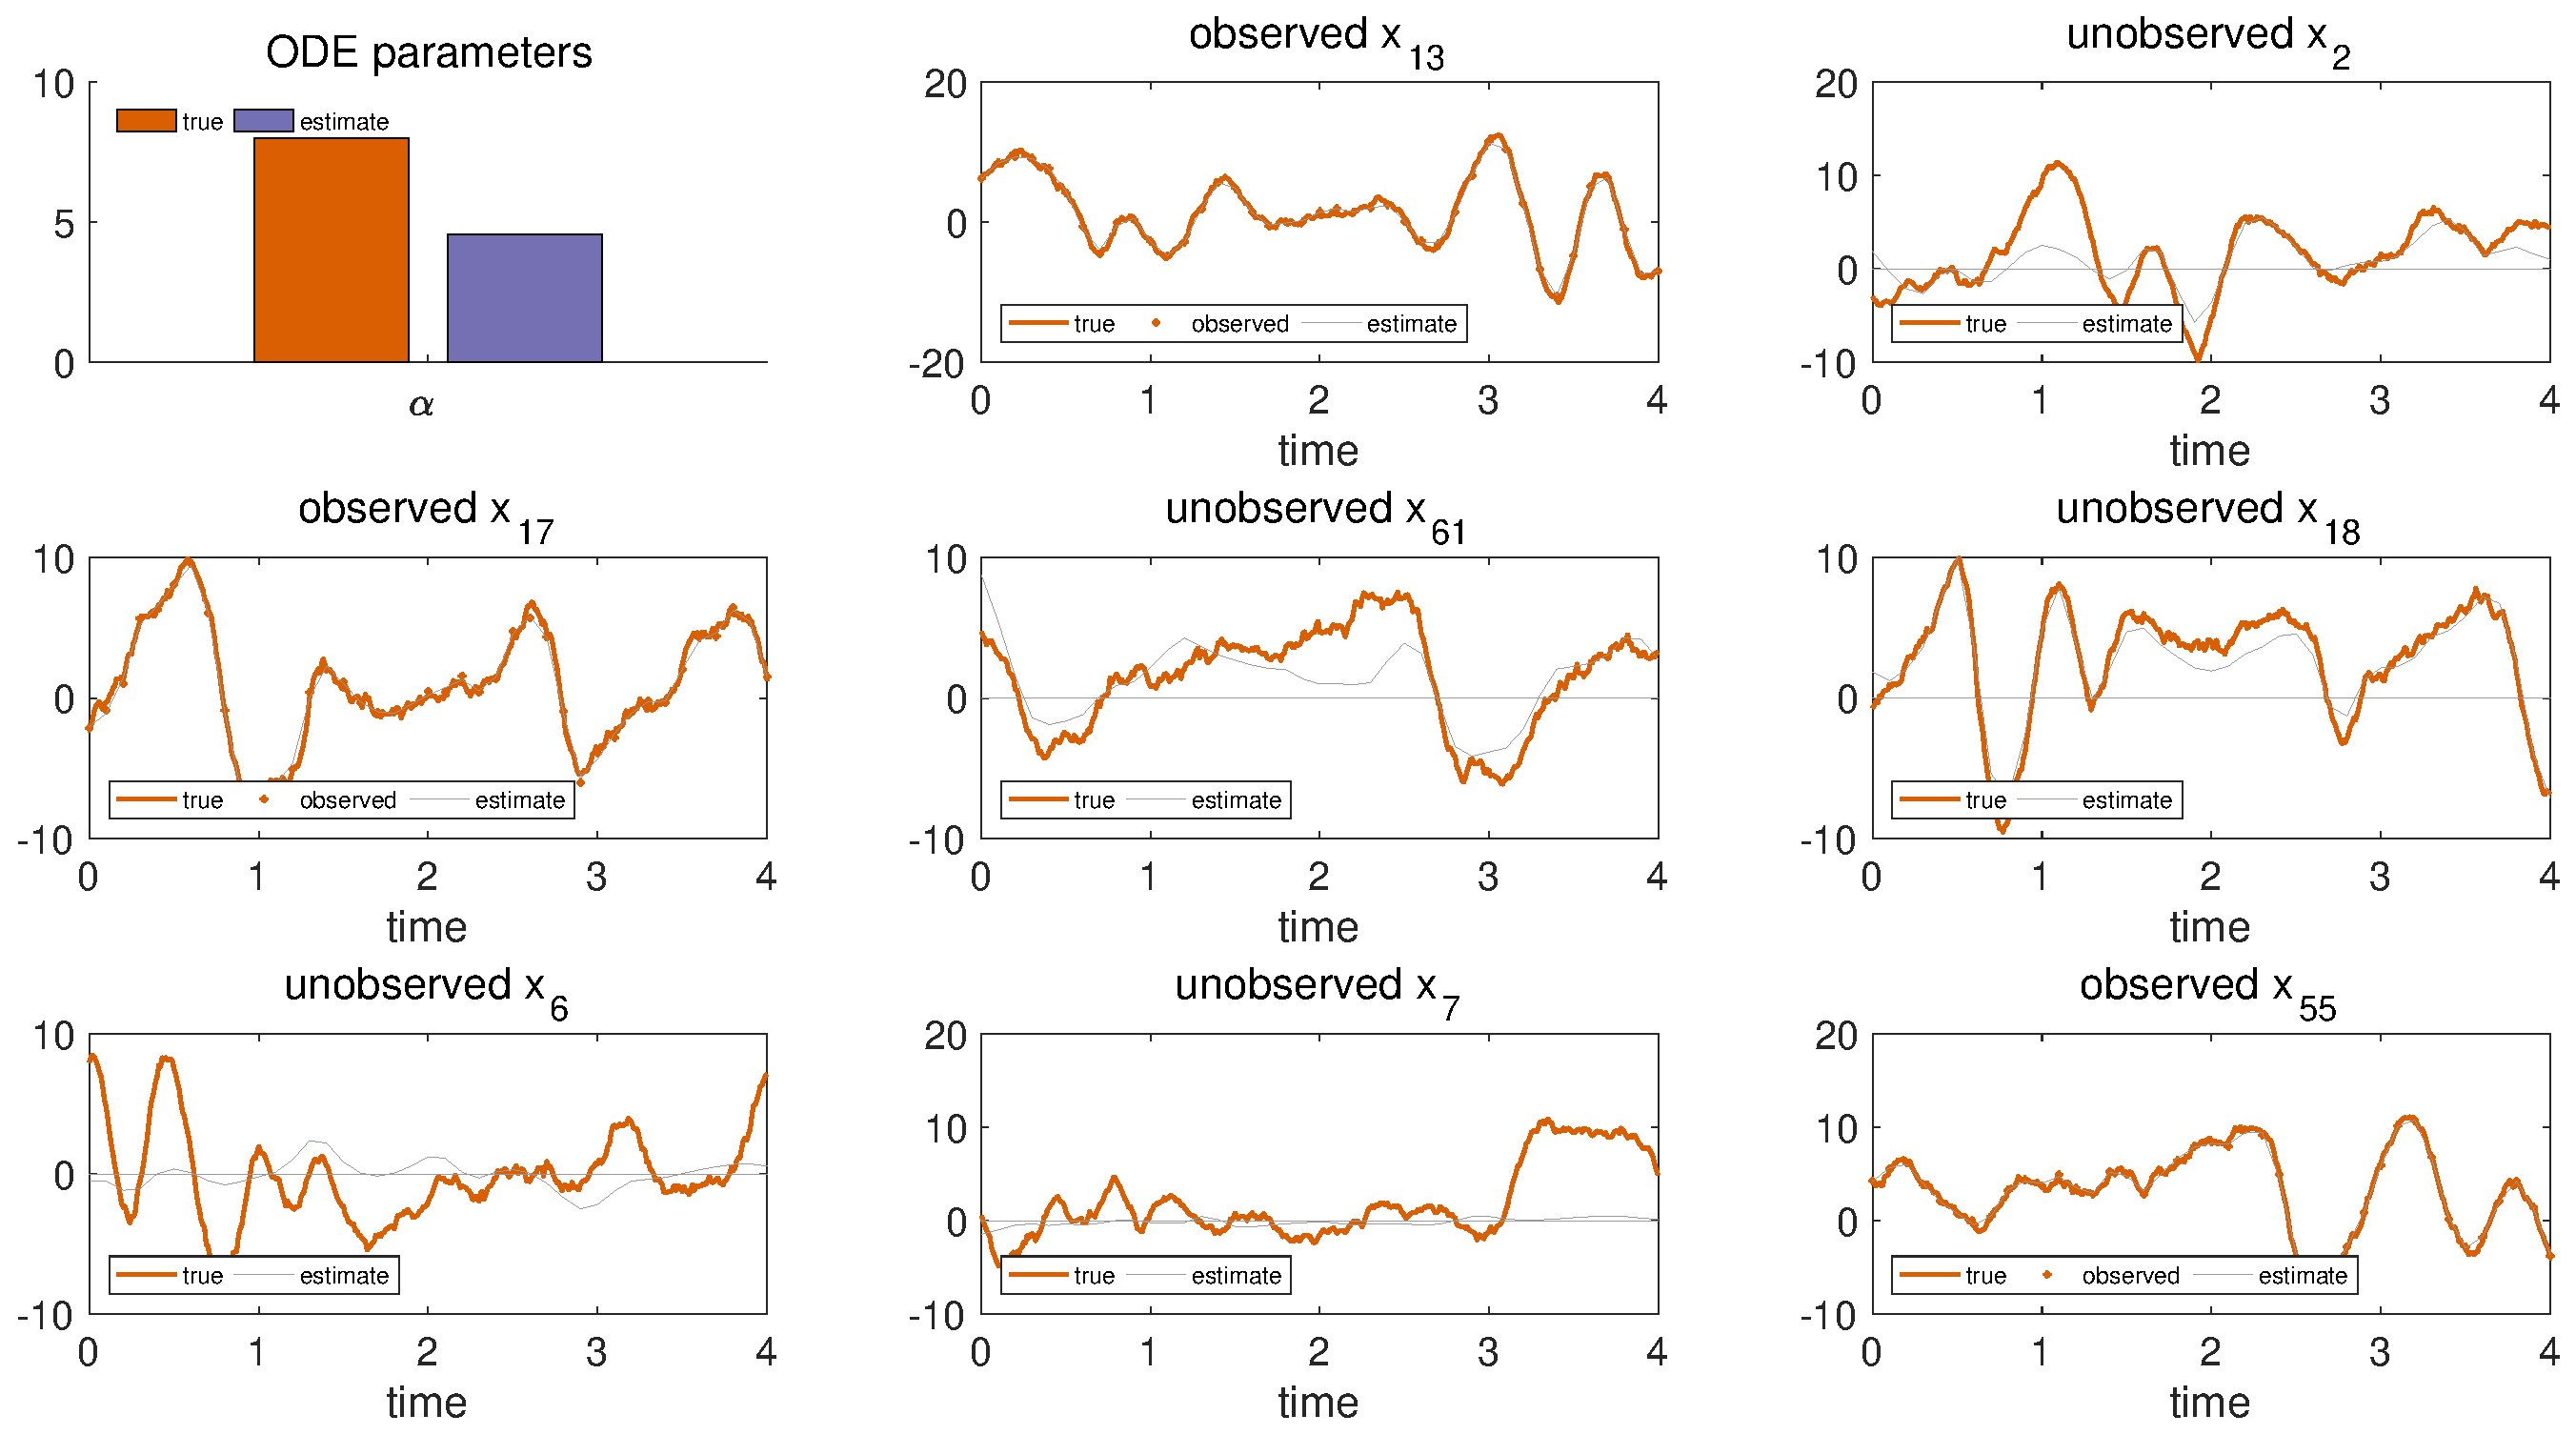
\includegraphics [width=4in]{VGM_for_Lorenz96_03.eps}

\includegraphics [width=4in]{VGM_for_Lorenz96_04.eps}

\includegraphics [width=4in]{VGM_for_Lorenz96_05.eps}

\includegraphics [width=4in]{VGM_for_Lorenz96_06.eps}

\includegraphics [width=4in]{VGM_for_Lorenz96_07.eps}

\includegraphics [width=4in]{VGM_for_Lorenz96_08.eps}

\includegraphics [width=4in]{VGM_for_Lorenz96_09.eps}

\includegraphics [width=4in]{VGM_for_Lorenz96_10.eps}

\includegraphics [width=4in]{VGM_for_Lorenz96_11.eps}

\includegraphics [width=4in]{VGM_for_Lorenz96_12.eps}

\includegraphics [width=4in]{VGM_for_Lorenz96_13.eps}

\includegraphics [width=4in]{VGM_for_Lorenz96_14.eps}

\includegraphics [width=4in]{VGM_for_Lorenz96_15.eps}

\includegraphics [width=4in]{VGM_for_Lorenz96_16.eps}

\includegraphics [width=4in]{VGM_for_Lorenz96_17.eps}

\includegraphics [width=4in]{VGM_for_Lorenz96_18.eps}

\includegraphics [width=4in]{VGM_for_Lorenz96_19.eps}

\includegraphics [width=4in]{VGM_for_Lorenz96_20.eps}

\includegraphics [width=4in]{VGM_for_Lorenz96_21.eps}
\begin{par}

\end{par} \vspace{1em}
\begin{itemize}
\setlength{\itemsep}{-1ex}
   \item \textbf{Proxy for individual states}
\end{itemize}

\begin{verbatim}               Expanding the proxy distribution in equation (12) over
the individual state $$\mathbf{x}_u$$:\end{verbatim}
    
\begin{verbatim}               $\hat{q}(\mathbf{x}_u) \stackrel{(a)}{\propto} \exp \left(
~ E_{Q_{-u}}  \ln ( p(\mathbf{x}_u \mid \mathbf\theta, \mathbf{X}_{-u},\mathbf\phi,\gamma)
p(\mathbf{x}_u  \mid\mathbf{Y},\mathbf\phi,\mathbf\sigma) ) ~ \right)\\ \qquad
~ \stackrel{(b)}{=} \exp\big( ~ E_{Q_{-u}} \ln     \mathcal{N}\left(\mathbf{x}_u
; -\mathbf{B}_{u}^+ \mathbf{b}_u,     ~\mathbf{B}_u^{+} ~ (\mathbf{A} + \mathbf{I}\gamma)
~     \mathbf{B}_u^{+T} \right) + E_{Q_{-u}} \ln    \mathcal{N}\left(\mathbf{x}_u
; \mathbf\mu_u(\mathbf{Y}), \mathbf\Sigma_u    \right) \big)\\ \qquad ~= \exp\big(
~ E_{Q_{-u}} \ln                \mathcal{N}\left(\mathbf{x}_u ; -\mathbf{B}_{u}^+
\mathbf{b}_u,                ~\mathbf{B}_u^{+} ~ (\mathbf{A} + \mathbf{I}\gamma)
~                \mathbf{B}_u^{+T} \right) + E_{Q_{-u}} \ln                \mathcal{N}\left(\mathbf{x}_u
; \mathbf\mu_u(\mathbf{Y}), \mathbf{\sigma}_u                \right) \big)$.\end{verbatim}
    
\begin{verbatim}               In (a) we decompose the full conditional nto an ODE-informed
distribution and a data-informed distribution and in (b) we substitute the ODE-informed
distribution $p(\mathbf{x}_u \mid \mathbf\theta, \mathbf{X}_{-u},\mathbf\phi,\gamma)$
with its density given by equation (8).\end{verbatim}
    \begin{verbatim}
            [state.proxy.mean{:,symbols.state_string},state.proxy.inv_cov] = proxy_for_ind_states(state.lin_comb,...
                state.proxy.mean{:,symbols.state_string},param_proxy_mean',dC_times_invC,coupling_idx.states,symbols,mu,...
                inv_sigma,simulation.observed_states,A_plus_gamma_inv,opt_settings);
\end{verbatim}
\begin{verbatim}
end
\end{verbatim}
\begin{par}

\end{par} \vspace{1em}
\begin{itemize}
\setlength{\itemsep}{-1ex}
   \item \textbf{Final result}
\end{itemize}
\begin{verbatim}
            plot_results(fig_handle,state.proxy,simulation,param_proxy_mean,plot_handle,symbols,plot_settings,'final');
\end{verbatim}

\includegraphics [width=4in]{VGM_for_Lorenz96_22.eps}


\subsection*{Time Taken}

\begin{verbatim}
disp(['time taken: ' num2str(toc) ' seconds'])
\end{verbatim}

        \color{lightgray} \begin{verbatim}time taken: 348.5171 seconds
\end{verbatim} \color{black}
    

\subsection*{References}

\begin{par}
*Gorbach, N.S. , Bauer, S. *and Buhmann, J.M., Scalable Variational Inference for Dynamical Systems. 2017a. Neural Information Processing Systems (NIPS). Link to NIPS paper \begin{verbatim}here\end{verbatim} and arxiv paper \begin{verbatim}here\end{verbatim}.
\end{par} \vspace{1em}
\begin{par}
\textbf{Bauer, S. , Gorbach, N.S.} and Buhmann, J.M., Efficient and Flexible Inference for Stochastic Differential Equations. 2017b. Neural Information Processing Systems (NIPS). Link to NIPS paper \begin{verbatim}here\end{verbatim}.
\end{par} \vspace{1em}
\begin{par}
Wenk, P., Gotovos, A., Bauer, S., Gorbach, N.S., Krause, A. and Buhmann, J.M., Fast Gaussian Process Based Gradient Matching for Parameters Identification in Systems of Nonlinear ODEs. 2018. In submission to Conference on Uncertainty in Artificial Intelligence (UAI). Link to arxiv paper \begin{verbatim}here\end{verbatim}.
\end{par} \vspace{1em}
\begin{par}
Calderhead, B., Girolami, M. and Lawrence. N.D., 2002. Accelerating Bayesian inference over nonlinear differential equation models. In Advances in Neural Information Processing Systems (NIPS) . 22.
\end{par} \vspace{1em}
\begin{par}
The authors in bold font have contributed equally to their respective papers.
\end{par} \vspace{1em}



\end{document}
    
